\chapter{Web-based Application}\label{chap:evaluation}

Using the algorithm we propose a system that will help cooking people transform the typical region's food from the original recipe to a new one that has a typical taste of specified region. For convenience and wider use, we develop this system as a web-based system. The system's outline and the model are described below.  

\section{The System's Outline} 

The system has two main functions:

\begin{itemize}

\item Suggesting possible recipes from the set of available materials inputted by the user. 

When people cook, they might already have many materials available in their house such as pepper, chili, chicken, etc. But they have no idea which food is the best choice to cook. Thus, we provide a system which has an extra function that accepts available materials inputted by users and then searches in the recipe database for recipes that are suitable for the inputted materials. ``Suitable'' means the number of extra-buy materials are the least. The suitable recipes will be shown in order; the smaller the number of extra-buy materials there are, the higher rank that recipe will be.

\item Transforming a recipe so that it has a specific region's taste. 

This is the most important function of the system. It uses the algorithm to extract the featured materials of the specified region and then transforms the original recipe to the new one. 
\end{itemize}

Based on these two functions we divide the system into three modules. These three modules are shown in the middle of Fig.~\ref{fig:system-model}, represented by three rectangle boxes. The model of the system is described in the next subsection.
 
\begin{figure*}[ht]
\centering
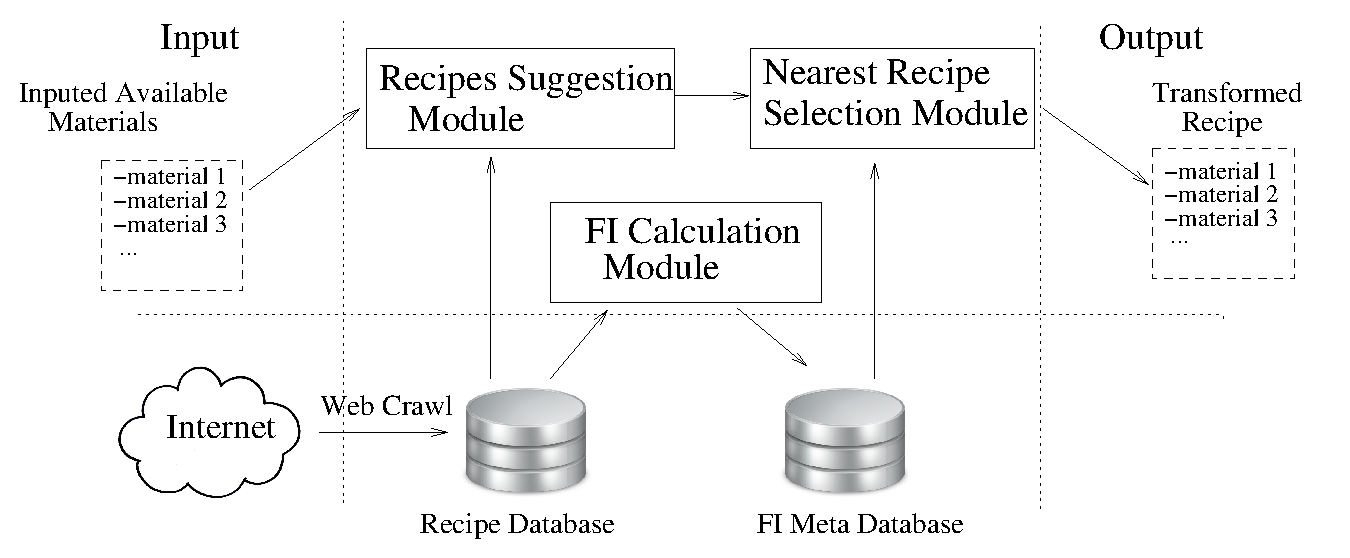
\includegraphics[scale=0.8]{system.eps} 
\caption{The System's Model with Recipe Suggestion Module, Featured Index Calculation Module and Nearest Recipe Selection Module.}
\label{fig:system-model}
\end{figure*}

\section{The System's Model}

\subsection{The Recipe Suggestion Module Based On Available Materials}

This module responds to the first function of the system, suggesting the possible recipes based on available materials inputted by the user. The input of this module is a set of available materials that the user has. It accesses the recipes database during the calculation and its output will be the list of the recipes which include most of the inputted materials. This output is passed to the Featured Index Calculation Module as shown in Fig.~\ref{fig:system-model}. After inputting available materials, the system will search in the recipe database for the most suitable recipes and show them in rank order. The pseudo code is shown as below. 

\begin{algorithmic}

\For{$recipe \in recipes$} 
\State $recipe.lack \gets |recipe| - |recipe \cup inputed\ materials|$
\EndFor

\State $sort\ the\ recipes\ by\ recipe.lack$

\Return $recipes$

\end{algorithmic}


\subsection{The Featured Index Calculation Module}

The user selects one of the recipes recommended by the Recipe Suggestion Module. Then selects the region which they want to transform the recipe in order to have that region's taste. This module applies the region's Featured Materials Extracting Algorithm and outputs the list of Featured Index for all materials in the region then stores them in the $FI$ Meta Database as shown in Fig.~\ref{fig:system-model}. Because we are not using all of the lists to extract the featured materials, we only look at two kinds of the following materials: 

\begin{itemize}
\item The top rank $FI$ materials.

These materials are the materials which are often used in the desired region, but not in other regions. 
\item The bottom rank $FI$ materials.

These materials are the most common materials which are used in almost all regions, but with different amounts. 
	 
\end{itemize}

We use both kinds and combine them with the materials appearing in the original recipe. The result is the list of materials and their amount for the food. The output should look in the shape as follows:

\begin{itemize}
\item Onion 2     (original)
\item Lemon 1/2   (original)
\item \ldots
\item Natto 100g  (top $FI$, newly added, region's average)
\item Sugar 100g  (bottom $FI$, newly added, region's average)
\end{itemize}

Among the bottom rank $FI$ materials, we only take the materials which are already in original recipe to apply into a new recipe. Among the newly added materials we use the average amount of them in the region. The output of this module is passed to the Nearest Recipe Selection Module. 
 
\subsection{The Nearest Recipe Selection Module} 

The output of Featured Index Calculation Module gives us the list of materials and their amount which is suitable for the region's taste. But it doesn't mean that we could use that list to make food. If we immediately apply the list of ingredients with the associated amount, we may have a wrong solution. This is because the newly added ingredients and their associated amounts are just the mean value of ingredients in the region. In result, there is the possibility of a bad tasting food. Thus, we propose to search in the region the nearest recipe in term of ingredients and amount. Then apply the suitable ingredients and its amount in that recipe to our food.        

Consider the list of materials as a vector. We calculate the similarity between the region's recipe and the average output above. Because we currently have ingredients and their amounts, there is the problem that the unit of ingredient's amounts are different and we cannot calculate the similarity. Thus we need to normalize these units. The alternative, we propose, is taking the fraction between the recipe's amount and the average amount all over the country. This gives us the values that are unit-independent, therefore usable for the similarity calculation. There are various methods to calculate the similarity between two vectors~\cite{cosine,euclidean,Qian:2004:SEC:967900.968151}. Among of these methods, Cosine similarity and Euclidean distance are the most famous methods. In this paper, we use the Euclidean distance, therefore the minimum value is adapted. The details of the algorithm is shown below. $X(x_1,x_2,\ldots,x_m)$ with $m \in N $ is the list outputted by the FI Calculation Module and $Y(y_1,y_2,\ldots,y_n)$ with $n \in N $ represents a list in the lists of the specified region's recipes 


\begin{algorithmic}

\For{$ingredient \in recipe\ X $} 
\State $ x_i \gets \frac{\displaystyle amount}{\displaystyle average\ amount\ in\ the\ country}$
\EndFor

\State $min \gets \infty $
\For{$recipe \in region's\ recipes$} 
\For{$ingredient \in recipe\ Y$} 
\State $ y_i \gets \frac{\displaystyle amount}{\displaystyle average\ amount\ in\ the\ country}$
\EndFor
\State $ similarity \gets \sqrt{\displaystyle \sum^l_{i=k}{(x_i-y_i)^2}}$
\If {$ similarity < min $}
\State $ min \gets similarity $
\EndIf
\EndFor

\Return $recipes$


\end{algorithmic}

Note that though $X$ and $Y$ don't have to have the same dimensions but we only select the ingredients $i$ which appears both in $X$ and $Y$ to calculate the similarity. $x_i$ and $y_i$ in which $i \in [k,l]$, are the amounts of ingredient $i$ in $X$ and $Y$ respectively.

\section{Database Design}


\subsection{Entity Relation Diagram}

Basically, we have the following entities:
\begin{itemize}
\item Entity of Ingredient mainly has attributes of ingredient such as: ingredient's name, ingredient's unit, ingredient's 
\item Entity of Recipe has recipe's name, introduction, instruction, image attributes.
\item Entity of User has user's name, email, password attributes.
\item Entity of Region has attributes of region's name, description about the region.
\end{itemize}

and the following relations between these entities:

\begin{itemize}
\item The relation named ``belong to'' between entity of recipe and region. Many recipes might belong to one region. This is a many-one relation. 
\item The relation named ``content'' between entity of recipe and ingredient. One recipe has many ingredient and one ingredient could appear in many recipe. This is a many-many relation. 
\item The relation named ``in'' between entity of user and entity region. The relation indicate which region the user is living in and it make a base to recognize the region of the newly registered by user. This is a many-one relation.
\item The relation named ``available'' between entity user and entity ingredient. As we describe in the previous sections, our system will have a function that allow user to register their available ingredients in their home and the system will recommend suitable recipes. A user might have many ingredients and one ingredient might appear in many user's home. Thus the relation here is many-many relation.
\item The relation named ``meta'' between entity of region and ingredient. This is the most important relation in our system because it reflects the algorithm. The meta data of $IF$, $FI$, $IA$ are included in this relation. Because these data are different from region to region and ingredient to ingredient. 
\end{itemize}


\begin{figure}
\centering
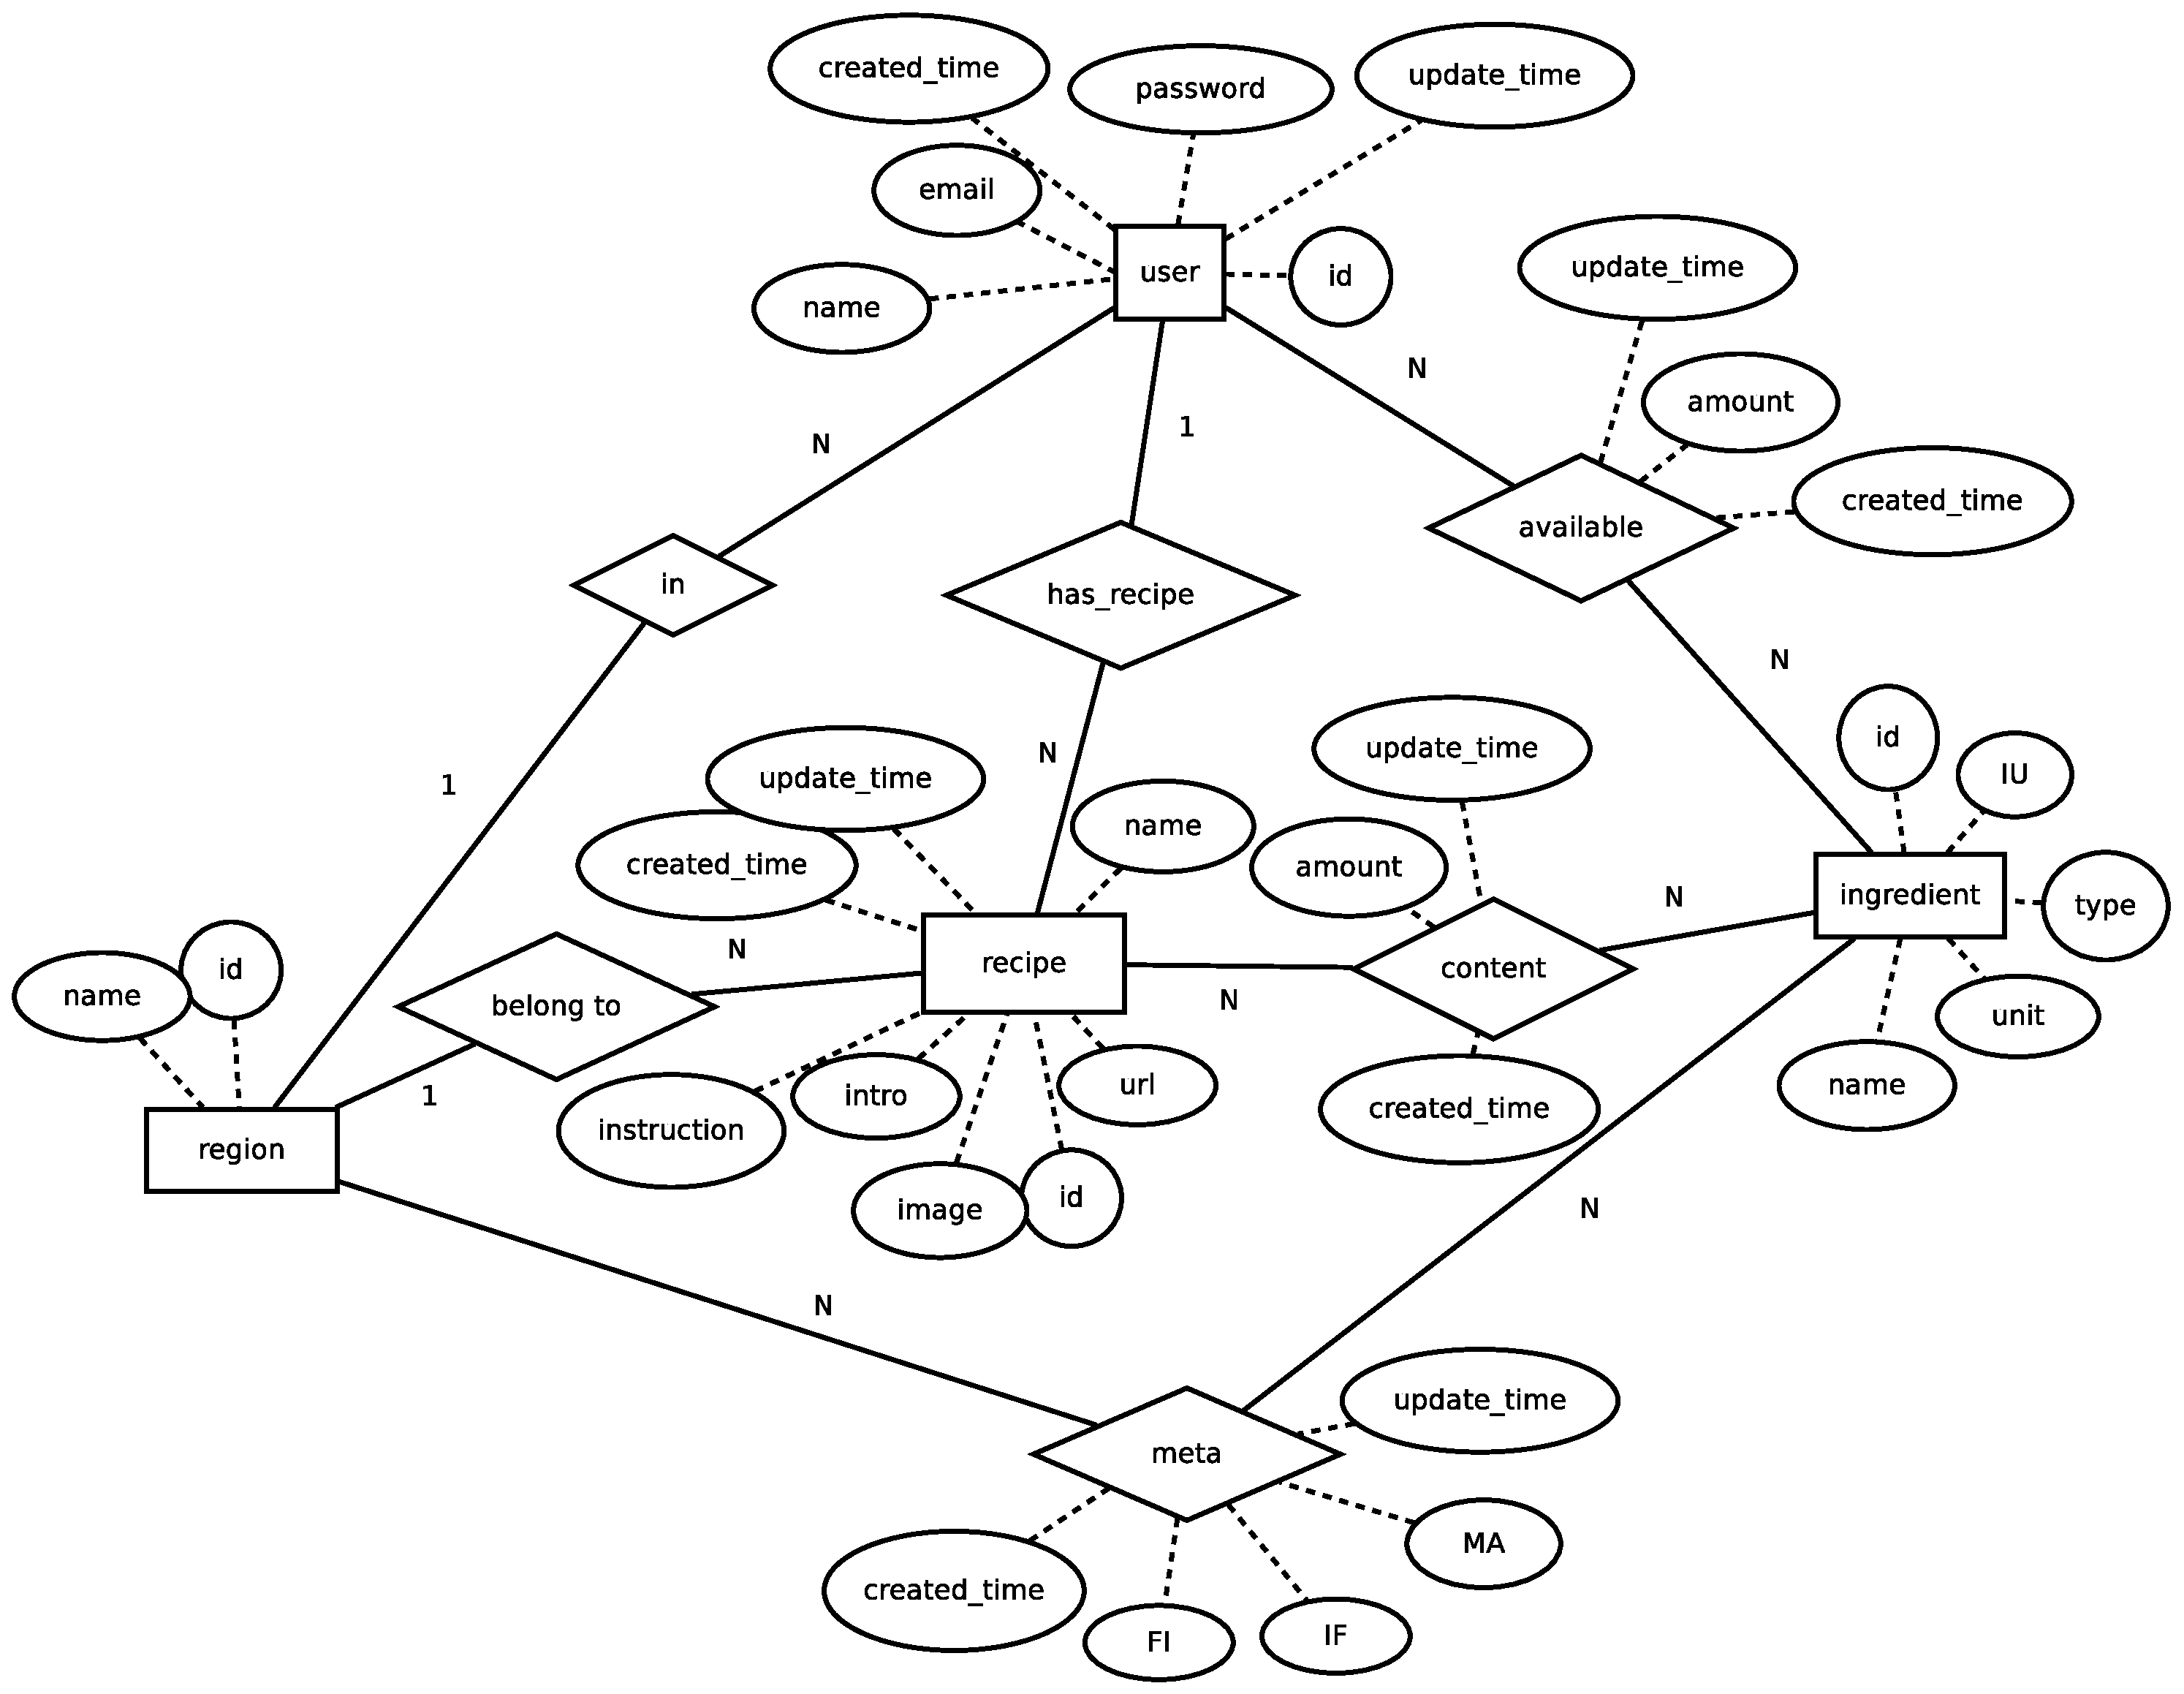
\includegraphics[scale=0.35]{ER.eps}
\caption{Entity Relation Diagram}
\label{fig:ER}

\end{figure}

The entities relations diagram of the system is shown in Fig.~\ref{fig:ER}

\subsection{Database Scheme}

After we have a entity relation diagram we turn it into scheme in relational database. For example, we use SQL in this research. Each entity we create a table with columns reflecting attributes of the entity. For example, we create a table user for the entity of user with columns username, password, email which are the attributes of the entity. For many-one relation such as the relation between user and region we don't need to create a table. Instead, we add the primary key of region to user table as a foreign key. For a many-many relation we create a new table that include both primary keys of two entities which are having the relation.

Fig.~\ref{fig:scheme} shows the scheme for the system's database based on proposed entities relation diagram.

\begin{figure}
\centering
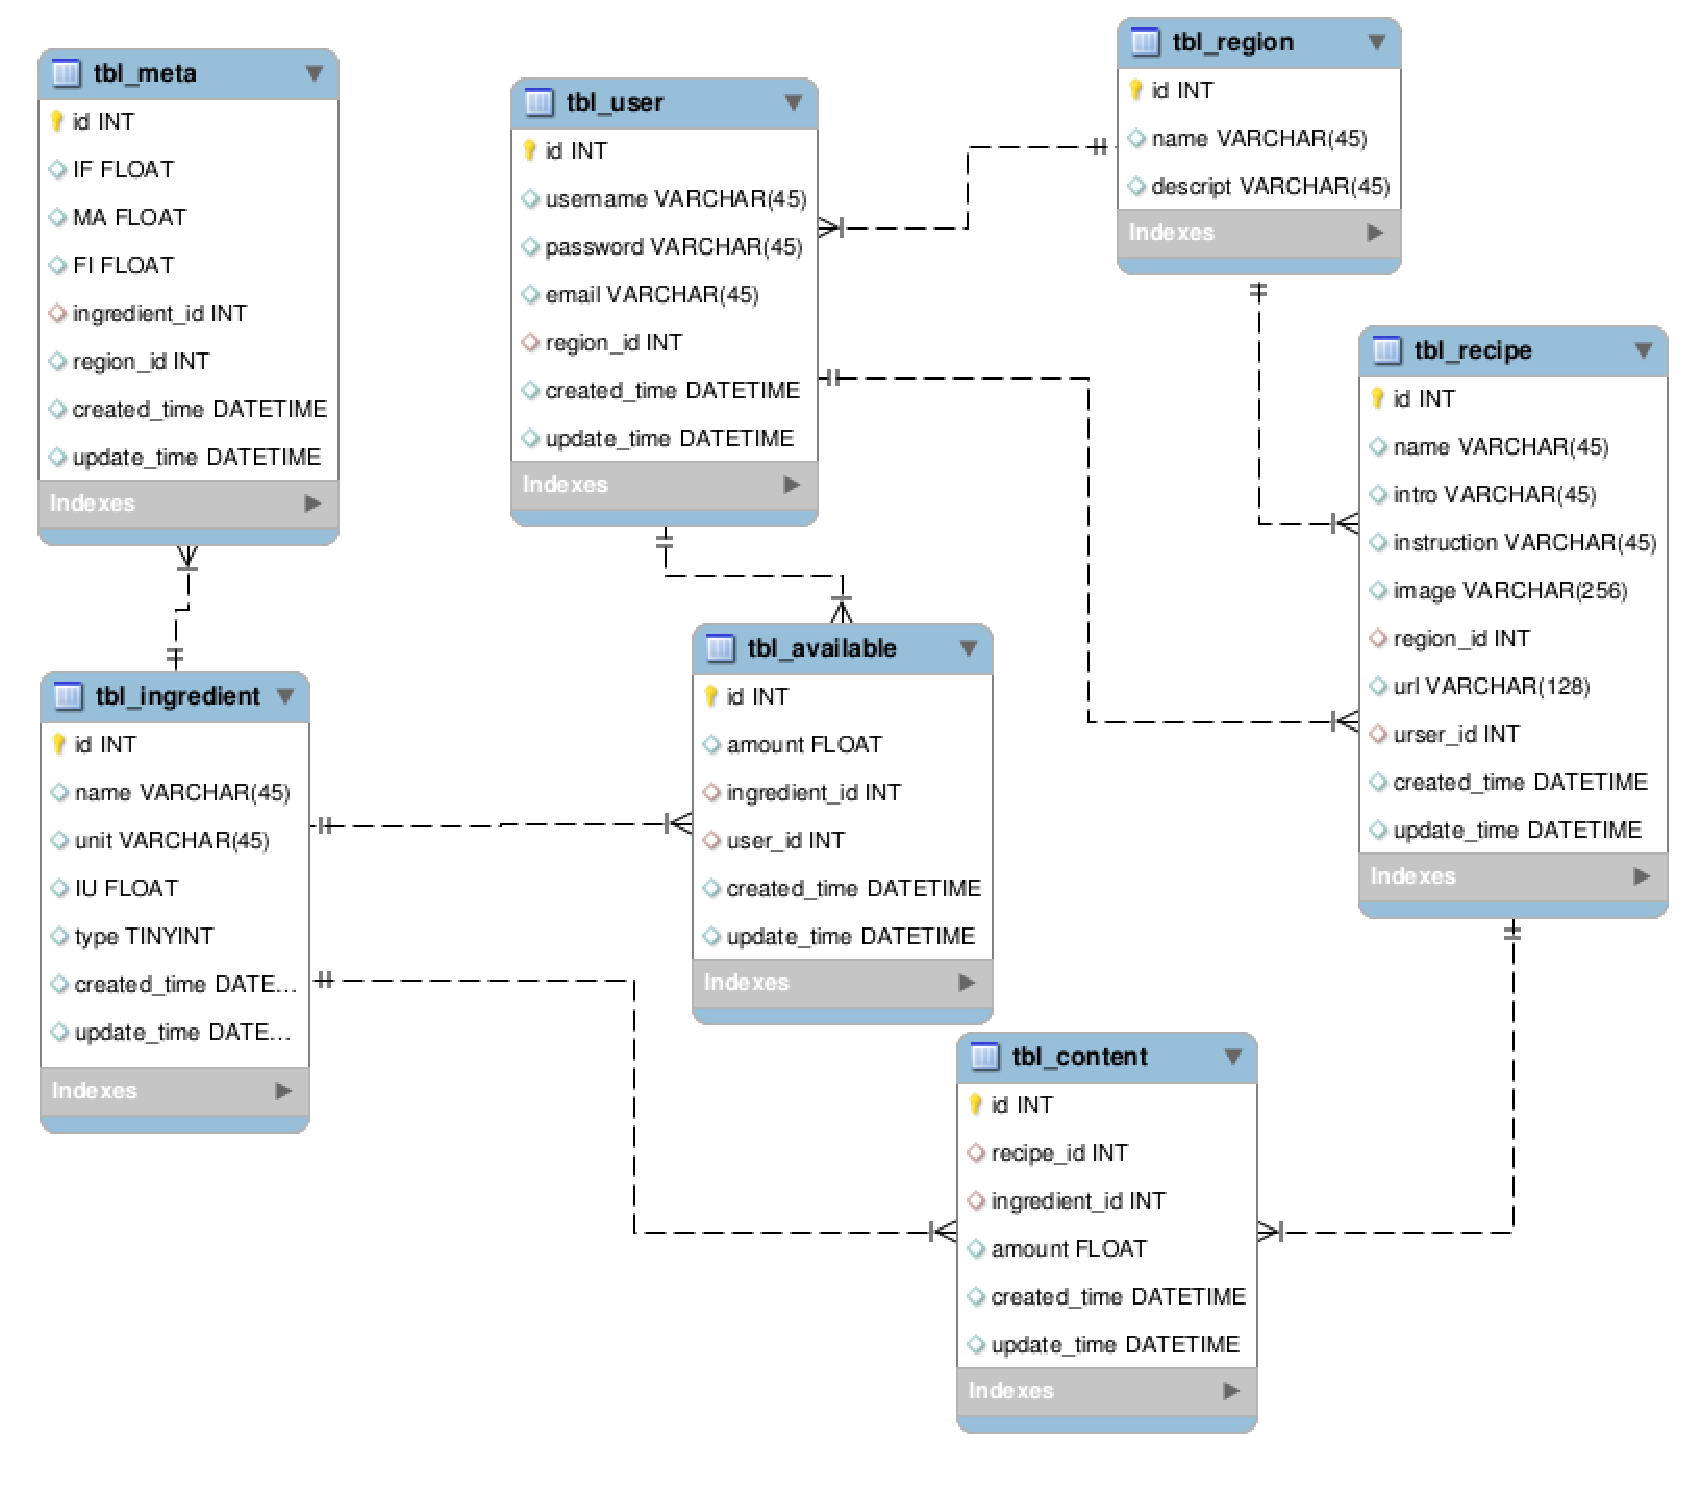
\includegraphics[scale=0.5]{scheme.eps}
\caption{Scheme for the System's Database}
\label{fig:scheme}

\end{figure}

\subsection{Database for real Data}

Fig.~\ref{fig:ingredient} shows the real data for ingredients in Japan's recipes. For each ingredient we have an $IU$ value of it. The value reflect uniqueness of the ingredient among regions in Japan. The amount is not included in the table because the amount of ingredient depends on in which recipe it appears.
 
\begin{figure}
\centering
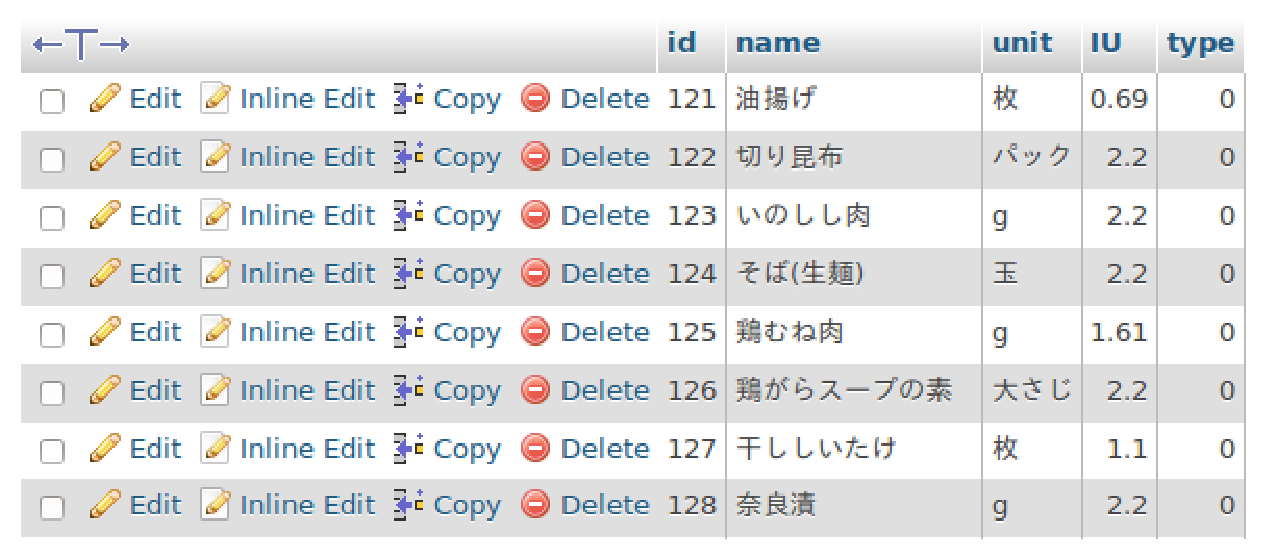
\includegraphics[scale=0.5]{ingredient.eps}
\caption{Ingredient Table with real data. It includes 404 ingredients.}
\label{fig:ingredient}
\end{figure}

The $TF$, $IA$, $MA$ and $IF$ value of ingredient are shown in Fig.~\ref{fig:ingredient}. We only use the $FI$ value for evaluating the featured ingredient but we also store the $TF$, $IA$, $MA$ value because they are necessary to recalculate the new meta data as we discussed in chapter 6, the Meta data recalculation section.



\section{Web Interfaces}


\begin{figure}
\centering
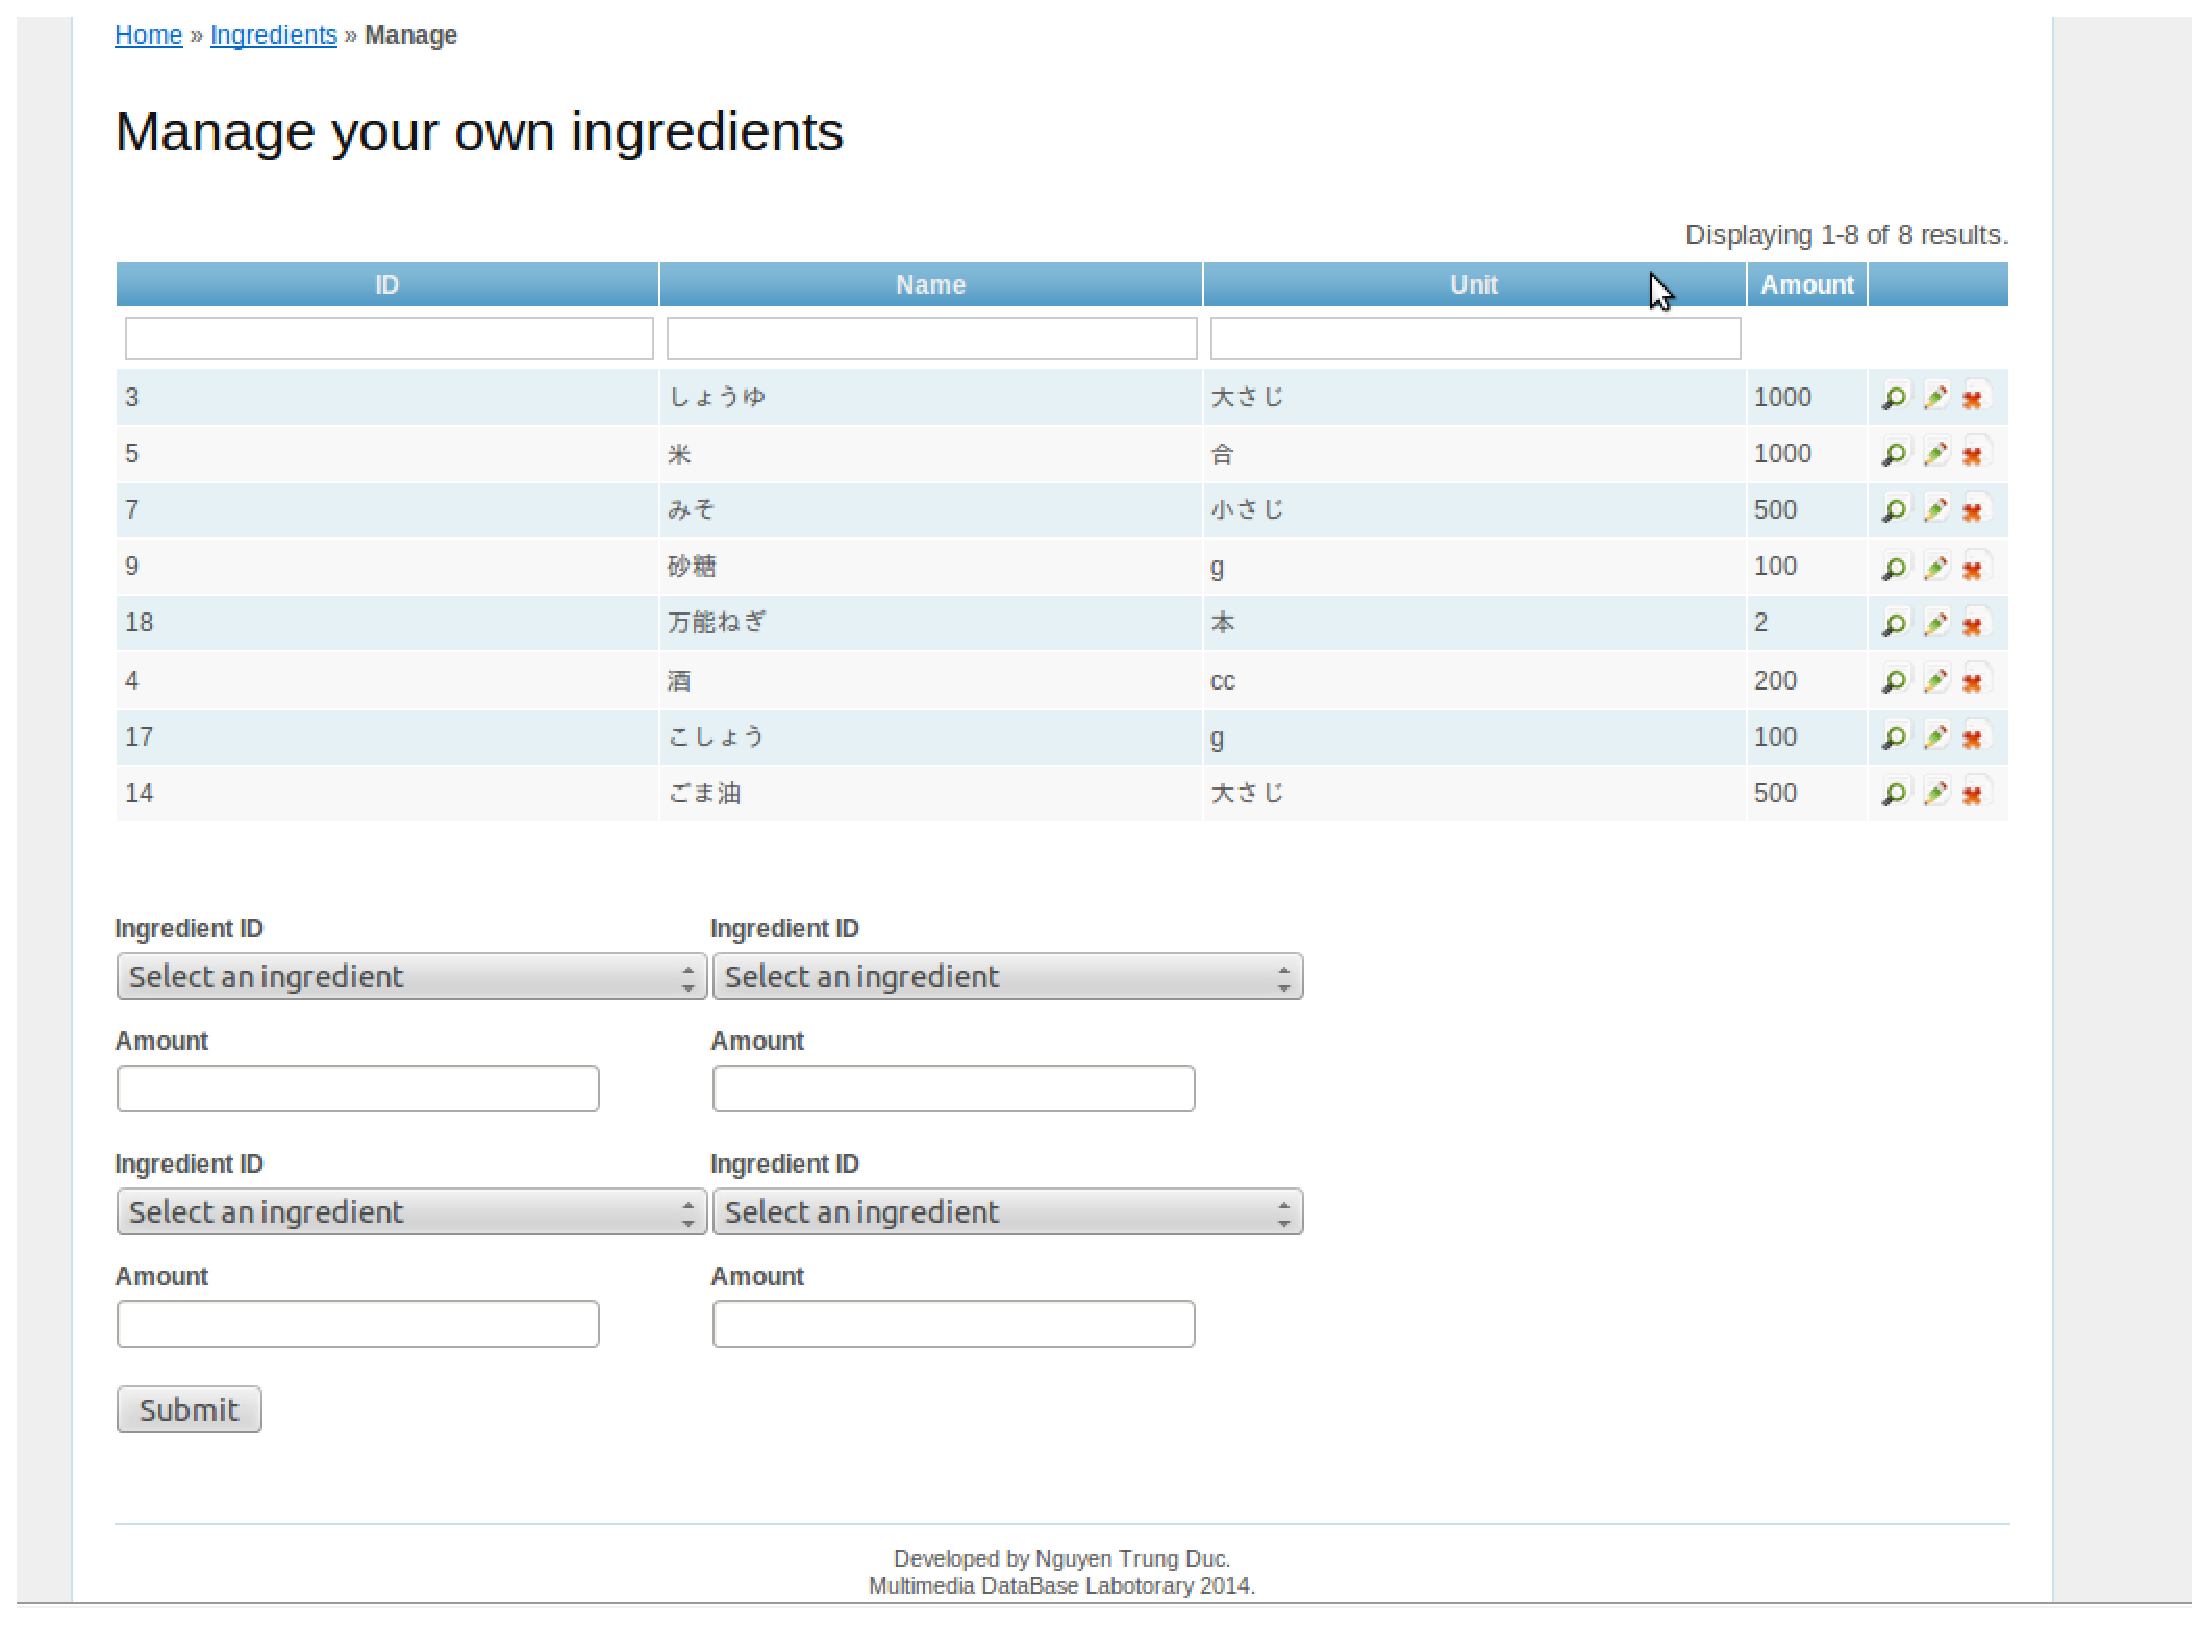
\includegraphics[scale=0.5]{your_ingredient.eps}
\caption{Page shows your home-available ingredients.}
\label{fig:your_ingredient}
\end{figure}

\begin{figure}
\centering
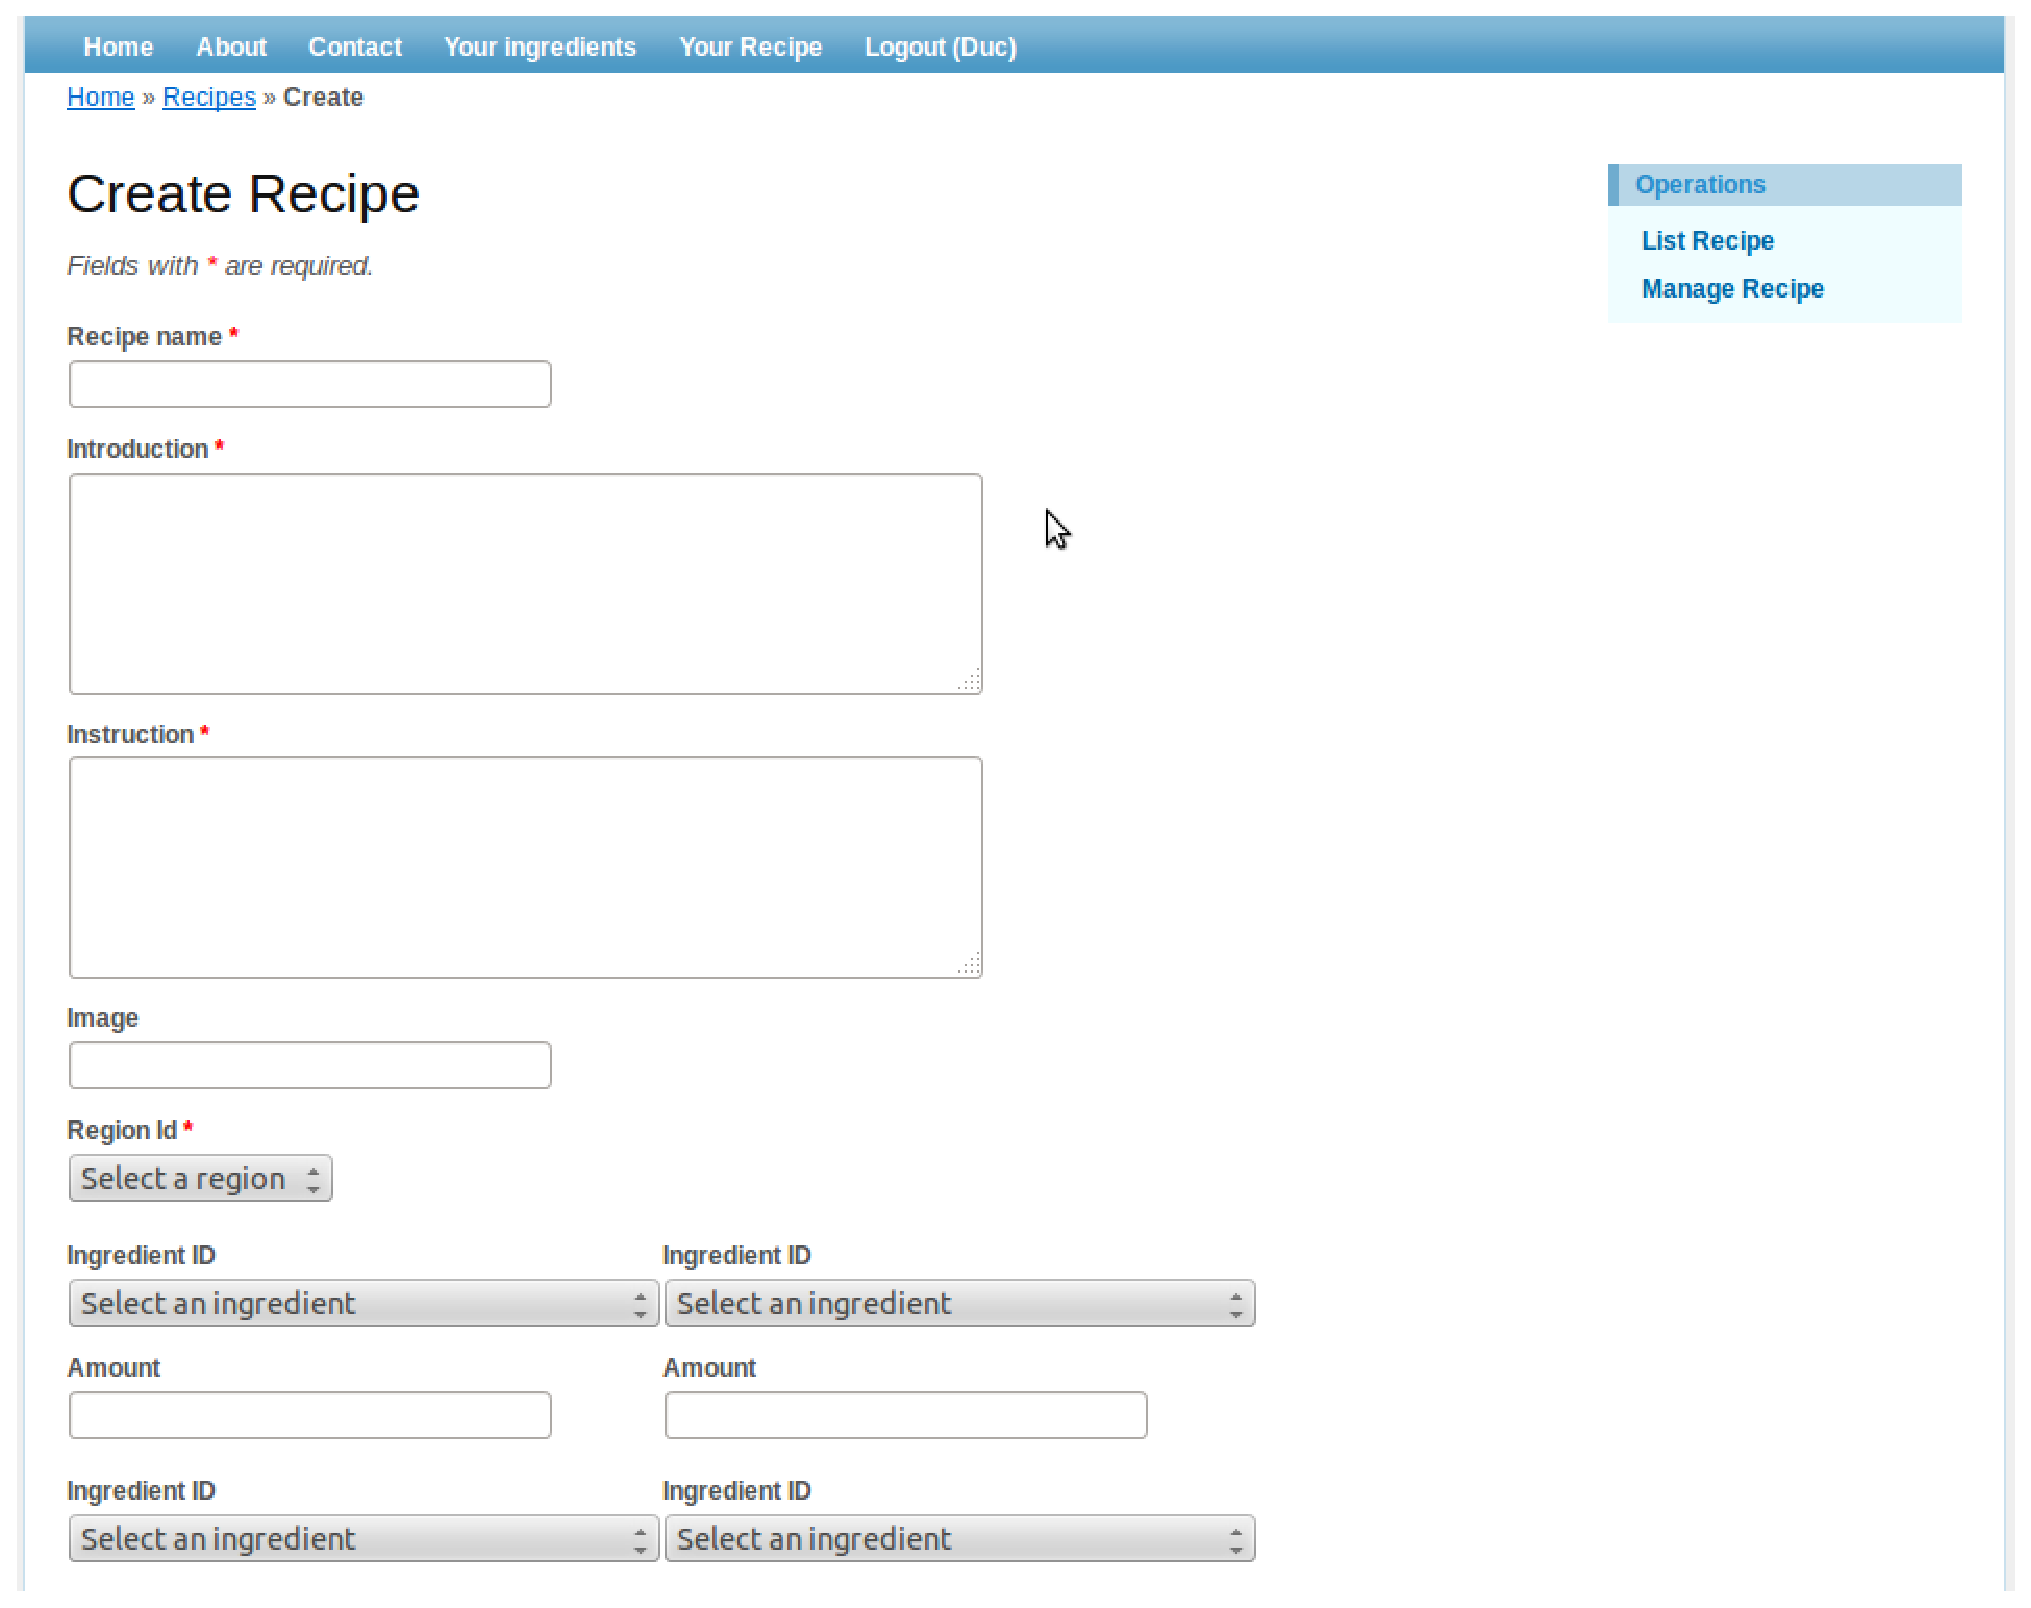
\includegraphics[scale=0.5]{register_recipe.eps}
\caption{Registering new recipe page.}
\label{fig:register_recipe}
\end{figure}

\begin{figure}
\centering
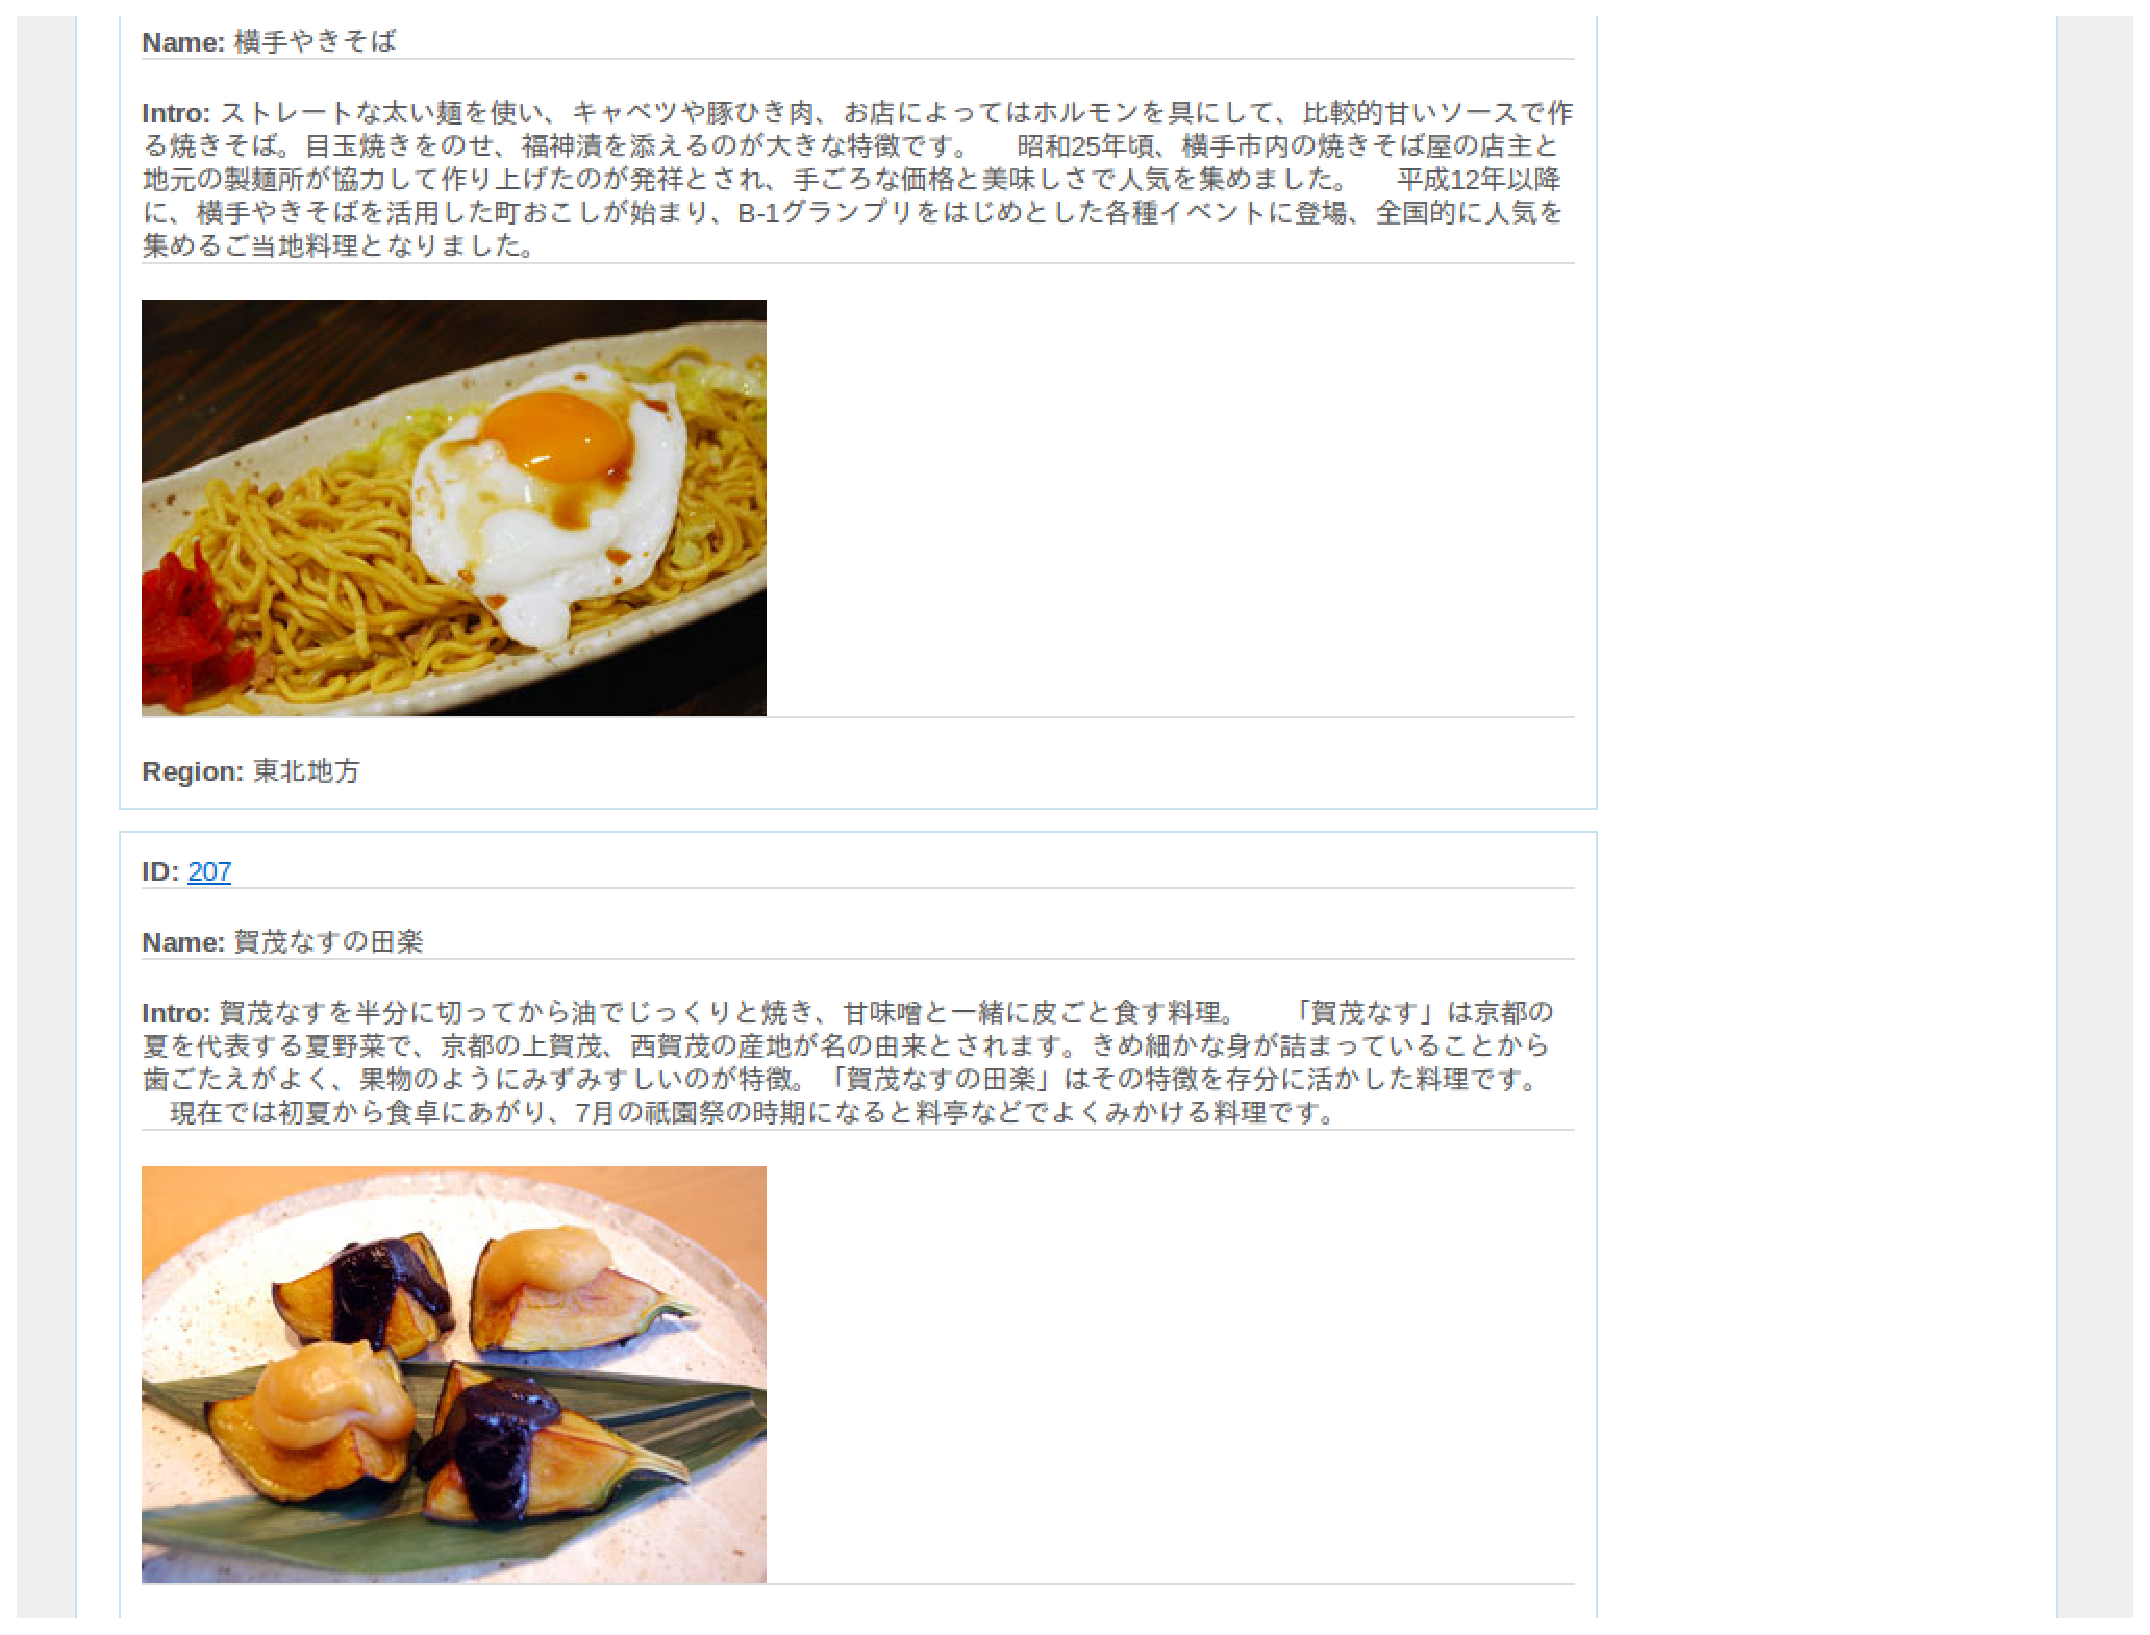
\includegraphics[scale=0.5]{your_recipe.eps}
\caption{Page shows your own recipes.}
\label{fig:your_recipe}
\end{figure}

\begin{figure}
\centering
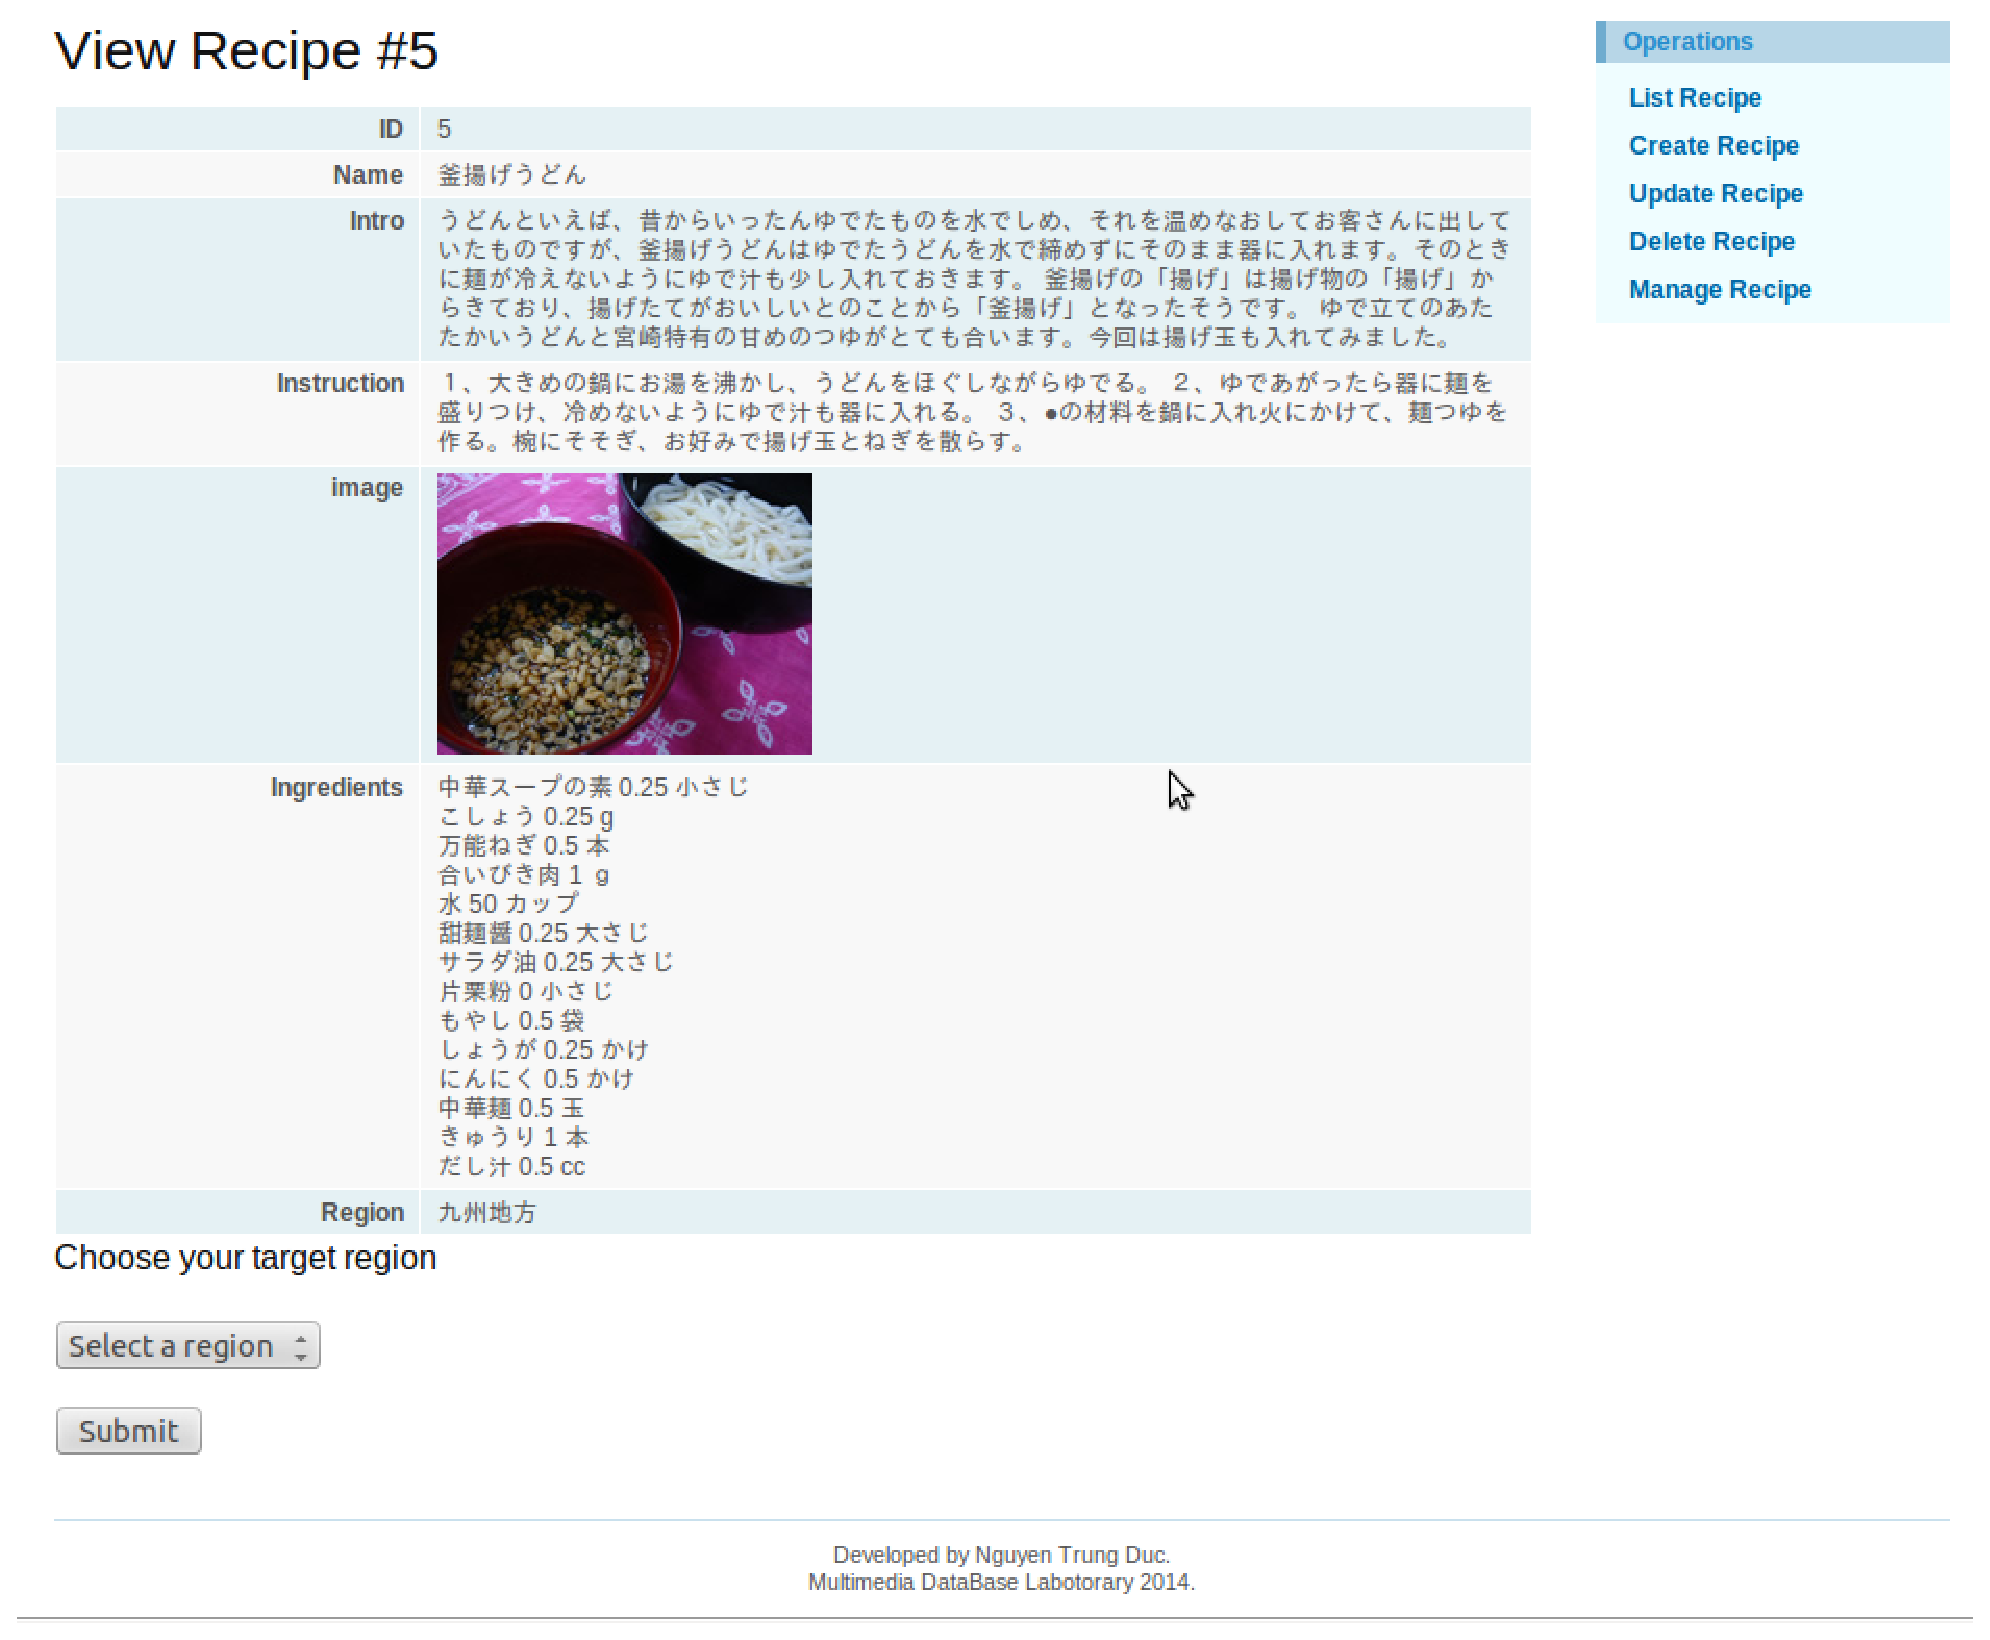
\includegraphics[scale=0.5]{choose_target.eps}
\caption{Choose the target region page.}
\label{fig:choose_target}
\end{figure}  
